
\section{Unified Virtual Layer}
The first problem is which space the virtual layer is implemented: kernel space or user space. Because container applications and virtual machines are both host processes, they can interact with the host kernel or other host processes. In addition, there are both user-level and kernel-level RNIC interface. Therefore, both kernel space and user space can realize the unified RDMA virtual layer. However, user space layer is friendly to containers because of lightweight and in favour of secure and flexible management. Moreover, software development in user space is less difficult, more portable and compatible. Therefore, uniRDMA chooses a user space virtual layer.

In traditional network virtualization, vNICs are virtulized and bridged to physical NIC, all vNICs are isolated but configed and manageed uniformly as a virtual network. Similarly, the main work of uniRDMA virtual layer is including vRNIC virtualization, vRNIC mapping  and virtual RDMA network management.The primary challenges are to make both isoaleted and high-performance for different vRNICs in the same virtual layer. 
	
\subsection{vRNIC Virtualization}
The RDMA resources is the key in both control path and data path at RDMA communication. In control path, the application creates queue instances such as QP, and registers memory regions(MRs) in host memory; In data path, the application writes DoorBell to notify RNIC to deal with WQE in QP and transform data in MRs.So, vRNIC virtulization is mainly about how to construct the virtual RDMA resoucrs to provide complete RDMA communication. We summarize that RNIC has two kinds of hardware properties about theses RDMA resources, namely static property and dynamic property:

For static properties,  since RDMA sends and receives messages based on QPs, MRs and other RDMA resources, it can be abstracted that the RDMA NIC has the following buffers inside:

\begin{itemize}
\item {\verb|Queue Buffer|}: storing information of queue instances, such as QP number, QP state and CQ number. The network card uses the information to read and write work requests, establish connections with remote QPs, etc.  
\item {\verb|Data Buffer|}: storing the information of registered memory regions, such as page table, memory key, etc. The network card use the informaation to access local or remote memory for data transform.  
\item {\verb|Doorbell Buffer|}: including multiple doorbell registers. The network card use it to accept user commands and notify the internal hardware processor to perform DMA, processing and forwarding. 
\end{itemize}

For dynamic attributes, Therefore, the state of RDMA resources are daynamic in control path and data path:  

\begin{itemize}
\item {\verb|Control Path|}: The creation and destruction of RDMA resources. RDMA resources or informations in buffer are always changed.For example, RNIC records the QP number when QP is created, changes QP state for RDMA connection and clear QP informations in the destory. Nofity that this porcess has losts latency due to the kernel .
\item {\verb|Data Path|}: The usage of RDMA resources.RDMA resources or informations in buffer are always maintained in RNIC. When RDMA applications post a send or receive operation, only write the DoorBell and the hardware processor performs DMA, encapsulates and forwards data.
\end{itemize}

To emulate the static attributes, virtual queue, data and doorbell buffers are respectively set up in vRNIC. For example, the QP buffer stores virtual QP information and the virtual doorbell buffer is include virtual doorbells. Virtual buffer is flexible and unlimited for the nums of RDMA resoucrs instances. 

To emulate the dynamic attributes, apparently, if only using pure software, it may cause low performance because of the software overhead in whole RDMA communication. Fortunately, we found all RDMA reources informations in RNIC are only changed in control path and maintained in data path. So, we can map the virtual RDMA reources to RNIC only in control path, such as QP and Doorbell,  and do not need introduce any operations in data path. Mapped RDMA resources are directly used and RNIC is notified by mapped virtual DoorBell in vRNIC. As a result, vRNIC are still with DMA zero-copy, hardware protocol stack processing and other high-performance capability in data path.

To realize this idea, we put each vRNIC with with a map unit. As Figure~\ref{fig:map-unit} shows, it maps or unmaps virtual RDMA resources from vRNIC to RNIC in control path:

\begin{figure}[!ht]
	\centering
	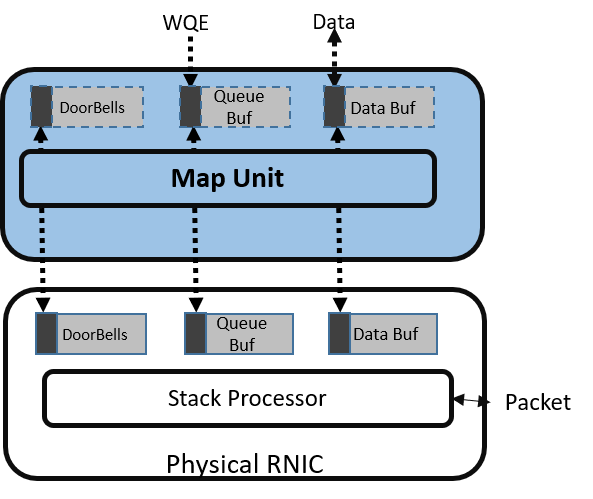
\includegraphics[width=1.0\linewidth]{images/map-unit}
	\caption{Map Unit in vRNIC}
	\label{fig:map-unit}
\end{figure}

\begin{itemize}
\item {\verb|For QPs, CQs and MRs|}: Taking QP as an example, regularly, vRNIC record virtual RDMA resources informations when the virtual QP instance are created. However, virtual QP are still not generated-associated with the RNIC. To make the maping, the map unit will create corresponding real QP instance in RNIC based on the information of virtual QP instances, such as the same memory address information and the same device id. Equivalently, the virtual QP informations are recongnized in RNIC, such as QP number and QP state, and can be one-to-one synchronous with RNIC's  physical instance by lots of similar map operations in control path. All operations can be completed by calling the Verbs interface of RNIC in user space. After the mapping is completed, the work requests in the vRNIC virtual QP can be zero-copied into the RNIC. Also, data in registered memroy of vRNIC can also be zero-copied to RNIC in the same way. 
\item {\verb|For DoorBells|}: It needs to be mapped to the hardware doorbell in the physical NIC device space, so that vRNIC has the ability to notify the RNIC hardware processors. In vRNIC, the mapping unit will map the virtual address of the virtual doorbell to the hardware doorbell address of the corresponding physical NIC device space through a system call. As shown in Figure 4-2, after the mapping is completed, the write operation to the vRNIC virtual doorbell is equivalent to performing the doorbell notification to the RNIC.
\end{itemize}

Map unit is the key for vRNICs' performance.Note that all mapping relationships are all one-to-one, therefore, the correctness and isolation of resources in different RDMA context are guaranteed. Meanwhile, because the mapping operation is only executed in control path, the overhead are one-off compared to data commands. For the data path, vRNICs can directly utilize the hardware processing capability of RNIC, such as DMA zero-copy and hardware protocol stack processing.

\subsection{vRNIC Mapping}
The same virtual layer needs to create multiple vRNICs and provide them to different containers or virtual machines respectively. If each vRNIC is directly mapped to the same RNIC, it will compete for the same PCIe bus and share the configuration space of RNIC. The vRNICs are still not isolated or limited.

SR-IOV is a popular hardware-based virtualization technology.RNIC can virtualize multiple different hardware interface, called VFs. Each VF has an unique PCIe bus and configuration space. At the same time, when configuring VFs, users can limit network rate and other hardware resources, and implement management policies such as QoS. The uniRDMA virtual layer maps each vRNIC to the VF interface of RNIC separately, so hardware-level isolation are guaranteed for vRNICs.

However, the VF resources of SR-IOV are limited, for example, only 126 VFs are supported in Mellanox ConnectX-3 at most. Therefore, the existing VFs need to be managed and coordinated in a unified to meet many vRNICs.

\begin{figure}[!ht]
	\centering
	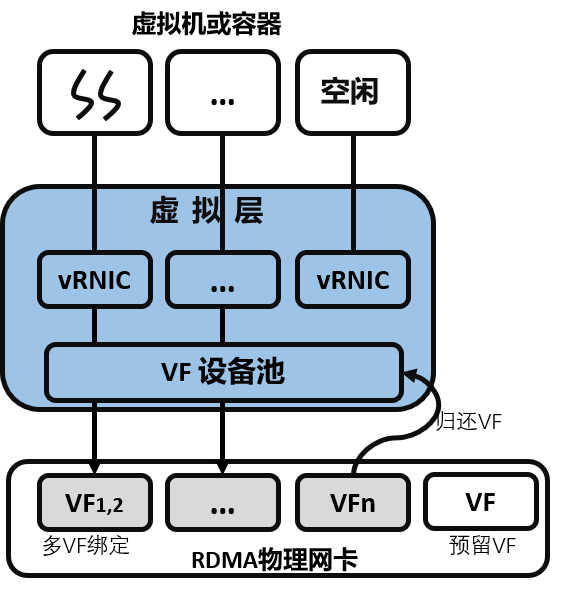
\includegraphics[width=1.0\linewidth]{images/vf-mapping}
	\caption{Management of vRNIC Mapping}
	\label{fig:vf-mapping}
\end{figure}

As Figure~\ref{fig:vf-mapping} shows: First, the virtual layer constructs a dynamic VF pool. The initial number of VFs in the pool is usually the number of pre-determined virtual instances. If lack of free VFs in the pool, the device pool can dynamically expand the number of VFs. Second, the virtual layer supports dynamic mapping between vRNIC and VF. When all virtual RDMA resources have been destroyed, the virtual layer marks the VF as idle and puts it back into the pool. So thatt the virtual layer can support the number of vRNICs that exceed the VF limit. Finally, the virtual layer supports various mapping relationships between vRNICs and VFs. For example, load balancing can be meeted by map a vRNIC with multipe VFs. VF resources are saved by mapping multiple vRNICs of the same virtual instance to the single VF. 

\subsection{Virtual RDMA Management}
To maintain portability and realize RDMA network management, RDMA connections between vRNICs can not be established by the physical address of VFs. But this problem has a solution that uniRDMA virtual layer acts as a software RDMA switch or router for virtual RDMA network configuration and routing management, etc.

RNICs are usually managed by the subnet manager in the cluster. For the same purpose, a control center is set up in uniRDMA to assign virtual RDMA addresses vGIDs to each vRNIC and configure routing rules between vRNICs. As shown in Figure~\ref{fig:route-config} , the vRNICs are divided into two groups: group 1 and group 2; vRNICs in the same group are allowed to establish RDMA connections, and cross-group RDMA connections can not succeed due to the isolated routing rules between group 1 and group 2.

\begin{figure}[!ht]
	\centering
	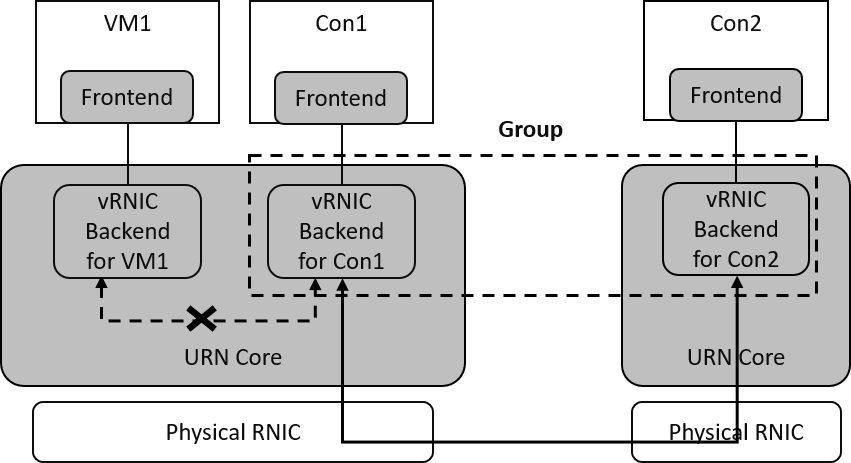
\includegraphics[width=1.0\linewidth]{images/route-config}
	\caption{Virtual RDMA Network Routing}
	\label{fig:route-config}
\end{figure}

Consistent with native RDMA, vRNICs in each virtual layer need to exchange each other's virtual RDMA addresses, virtual QP queue information, registered memory keys and other information to establish virtual RDMA connections. However, the vRNIC RDMA address is virtual, and does not recognized in RNIC. Therefore, the mapping relations between the virtual addresses of vRNICs and the physical addresses of VF needs to be exchanged between virtual layers. When establishing the virtual RDMA connection, the virtual RDMA address is converted to the physical address of the mapped VFs. Note that RDMA resources informations, such as virtual QP number and memory keys, have been mapped to the VF interface by the map unit in vRNIC, they can all be recognized VF and directly used to create RDMA connection.
